
%(BEGIN_QUESTION)
% Copyright 2010, Tony R. Kuphaldt, released under the Creative Commons Attribution License (v 1.0)
% This means you may do almost anything with this work of mine, so long as you give me proper credit

This is a pressure alarm circuit, designed to energize a warning light if the process pressure sensed by the pressure switch ever crosses a certain threshold value:

$$\includegraphics[width=15.5cm]{i04508x01.eps}$$

First, determine if this is a {\it low-pressure} alarm or a {\it high-pressure alarm} (i.e. under what type of process pressure condition will the light bulb energize, an abnormally low pressure or an abnormally high pressure?).

\vskip 20pt

Next, determine the effect of a bad wire connection (``open'' fault) at terminal 2 of the control relay on the status of the warning light.

\vskip 20pt \vbox{\hrule \hbox{\strut \vrule{} {\bf Suggestions for Socratic discussion} \vrule} \hrule}

\begin{itemize}
\item{} Identify how the circuit could be altered to alarm in the opposite condition it does now (i.e. high pressure instead of low pressure, or low pressure instead of high pressure, whichever you have determined the circuit to be in its present configuration). 
\end{itemize}

\underbar{file i04508}
%(END_QUESTION)





%(BEGIN_ANSWER)


%(END_ANSWER)





%(BEGIN_NOTES)

This is a {\bf low-pressure} alarm circuit.

\vskip 10pt

The consequence of this wiring fault is that the warning light will {\bf never come on}.

\vskip 20pt \vbox{\hrule \hbox{\strut \vrule{} {\bf Virtual Troubleshooting} \vrule} \hrule}

This question is a good candidate for a ``Virtual Troubleshooting'' exercise.  Presenting the diagram to students, you first imagine in your own mind a particular fault in the system.  Then, you present one or more symptoms of that fault (something noticeable by an operator or other user of the system).  Students then propose various diagnostic tests to perform on this system to identify the nature and location of the fault, as though they were technicians trying to troubleshoot the problem.  Your job is to tell them what the result(s) would be for each of the proposed diagnostic tests, documenting those results where all the students can see.

During and after the exercise, it is good to ask students follow-up questions such as:

\begin{itemize}
\item{} What does the result of the last diagnostic test tell you about the fault?
\item{} Suppose the results of the last diagnostic test were different.  What then would that result tell you about the fault?
\item{} Is the last diagnostic test the best one we could do?
\item{} What would be the ideal order of tests, to diagnose the problem in as few steps as possible?
\end{itemize}

%INDEX% Pictorial circuit review (relay circuit)

%(END_NOTES)


